\subsection{Videooptagelser}
\label{VideooptagelserValgAfGestikker}
%
I følgende afsnit vil de visuelle repræsentationer af de udvalgt gestikker blive udarbejdet. Der udarbejdes tre videoer; én hvor de udvalgte semaforiske gestikker til pause og start fremgår, én hvor de udvalgte semaforiske gestikke til at skifte musiknummer frem og tilbage fremgår og én hvor de udvalgte semaforiske gestikker til at skrue op og ned for musikken fremgår. Videooptagelserne redigeres i Windows Movie Maker version 2012 og de tre færdigredigerede videooptagelser fremgår i \textbf{elektroniske bilag}. 
\blankline
%
Fælles for de tre videooptagelser er, at de er optaget med et Canon Powershot s110 kamera på et stativ, kameraet optager både billede og lyd, optagelserne er taget med en 45$^{\circ}$'s vinkel i et halvnært perspektiv samt en neutral hvid baggrund og et neutralt ansigtsudtryk, hvilket er illustreret på \autoref{fig:Tryk}. Ved at optage med en 45$^{\circ}$'s vinkel i et halvnært perspektiv er det muligt at tydeliggøre størrelse, bevægelsesretning og dybde for hver af de udvalgte semaforiske gestikker. Ydermere tillader en 45$^{\circ}$'s vinkel at forstyrrelser i form af øjenkontakt mellem testperson og demonstratoren i optagelserne, minimeres. 
%
\begin{figure}[H]
	\centering
	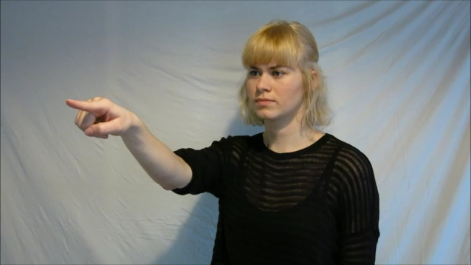
\includegraphics[resolution=300,width=\textwidth]{Test1/Tryk}
	\caption{Illustration af hvordan optagelserne foretages, med 45$^{\circ}$'s vinkel i et halvnært perspektiv samt en neutral hvid baggrund og et neutralt ansigtsudtryk.}
	\label{fig:Tryk}
\end{figure}
\noindent
%
Under optagelserne afspilles der musik fra en computer. Musiknummeret til at pause og starte musikken er \enquote{Stay} fra Zedd og Alessia Cara (2017). Musiknumrene til at skifte sang frem og tilbage er \enquote{Closer} fra The Chainsmokers ft. Halsey (2016) og \enquote{Galway Girl} fra Ed Sheeran (2017). Musiknummeret til at skrue op og ned for musikken er \enquote{You Don't Know Me} fra Jax Jones ft. RAYE (2017). Når der eksempelvis laves en gestik for at pause musikken, pauses musikken på computeren, for på den måde at demonstrerer hvilken gestik, der skal til for at musikken pauses. De resterende funktioner optages på tilsvarende måde.\blankline
%   
MANGLER FLOW for optagelser!\blankline
%
%
\begin{figure}[H]
	\centering
	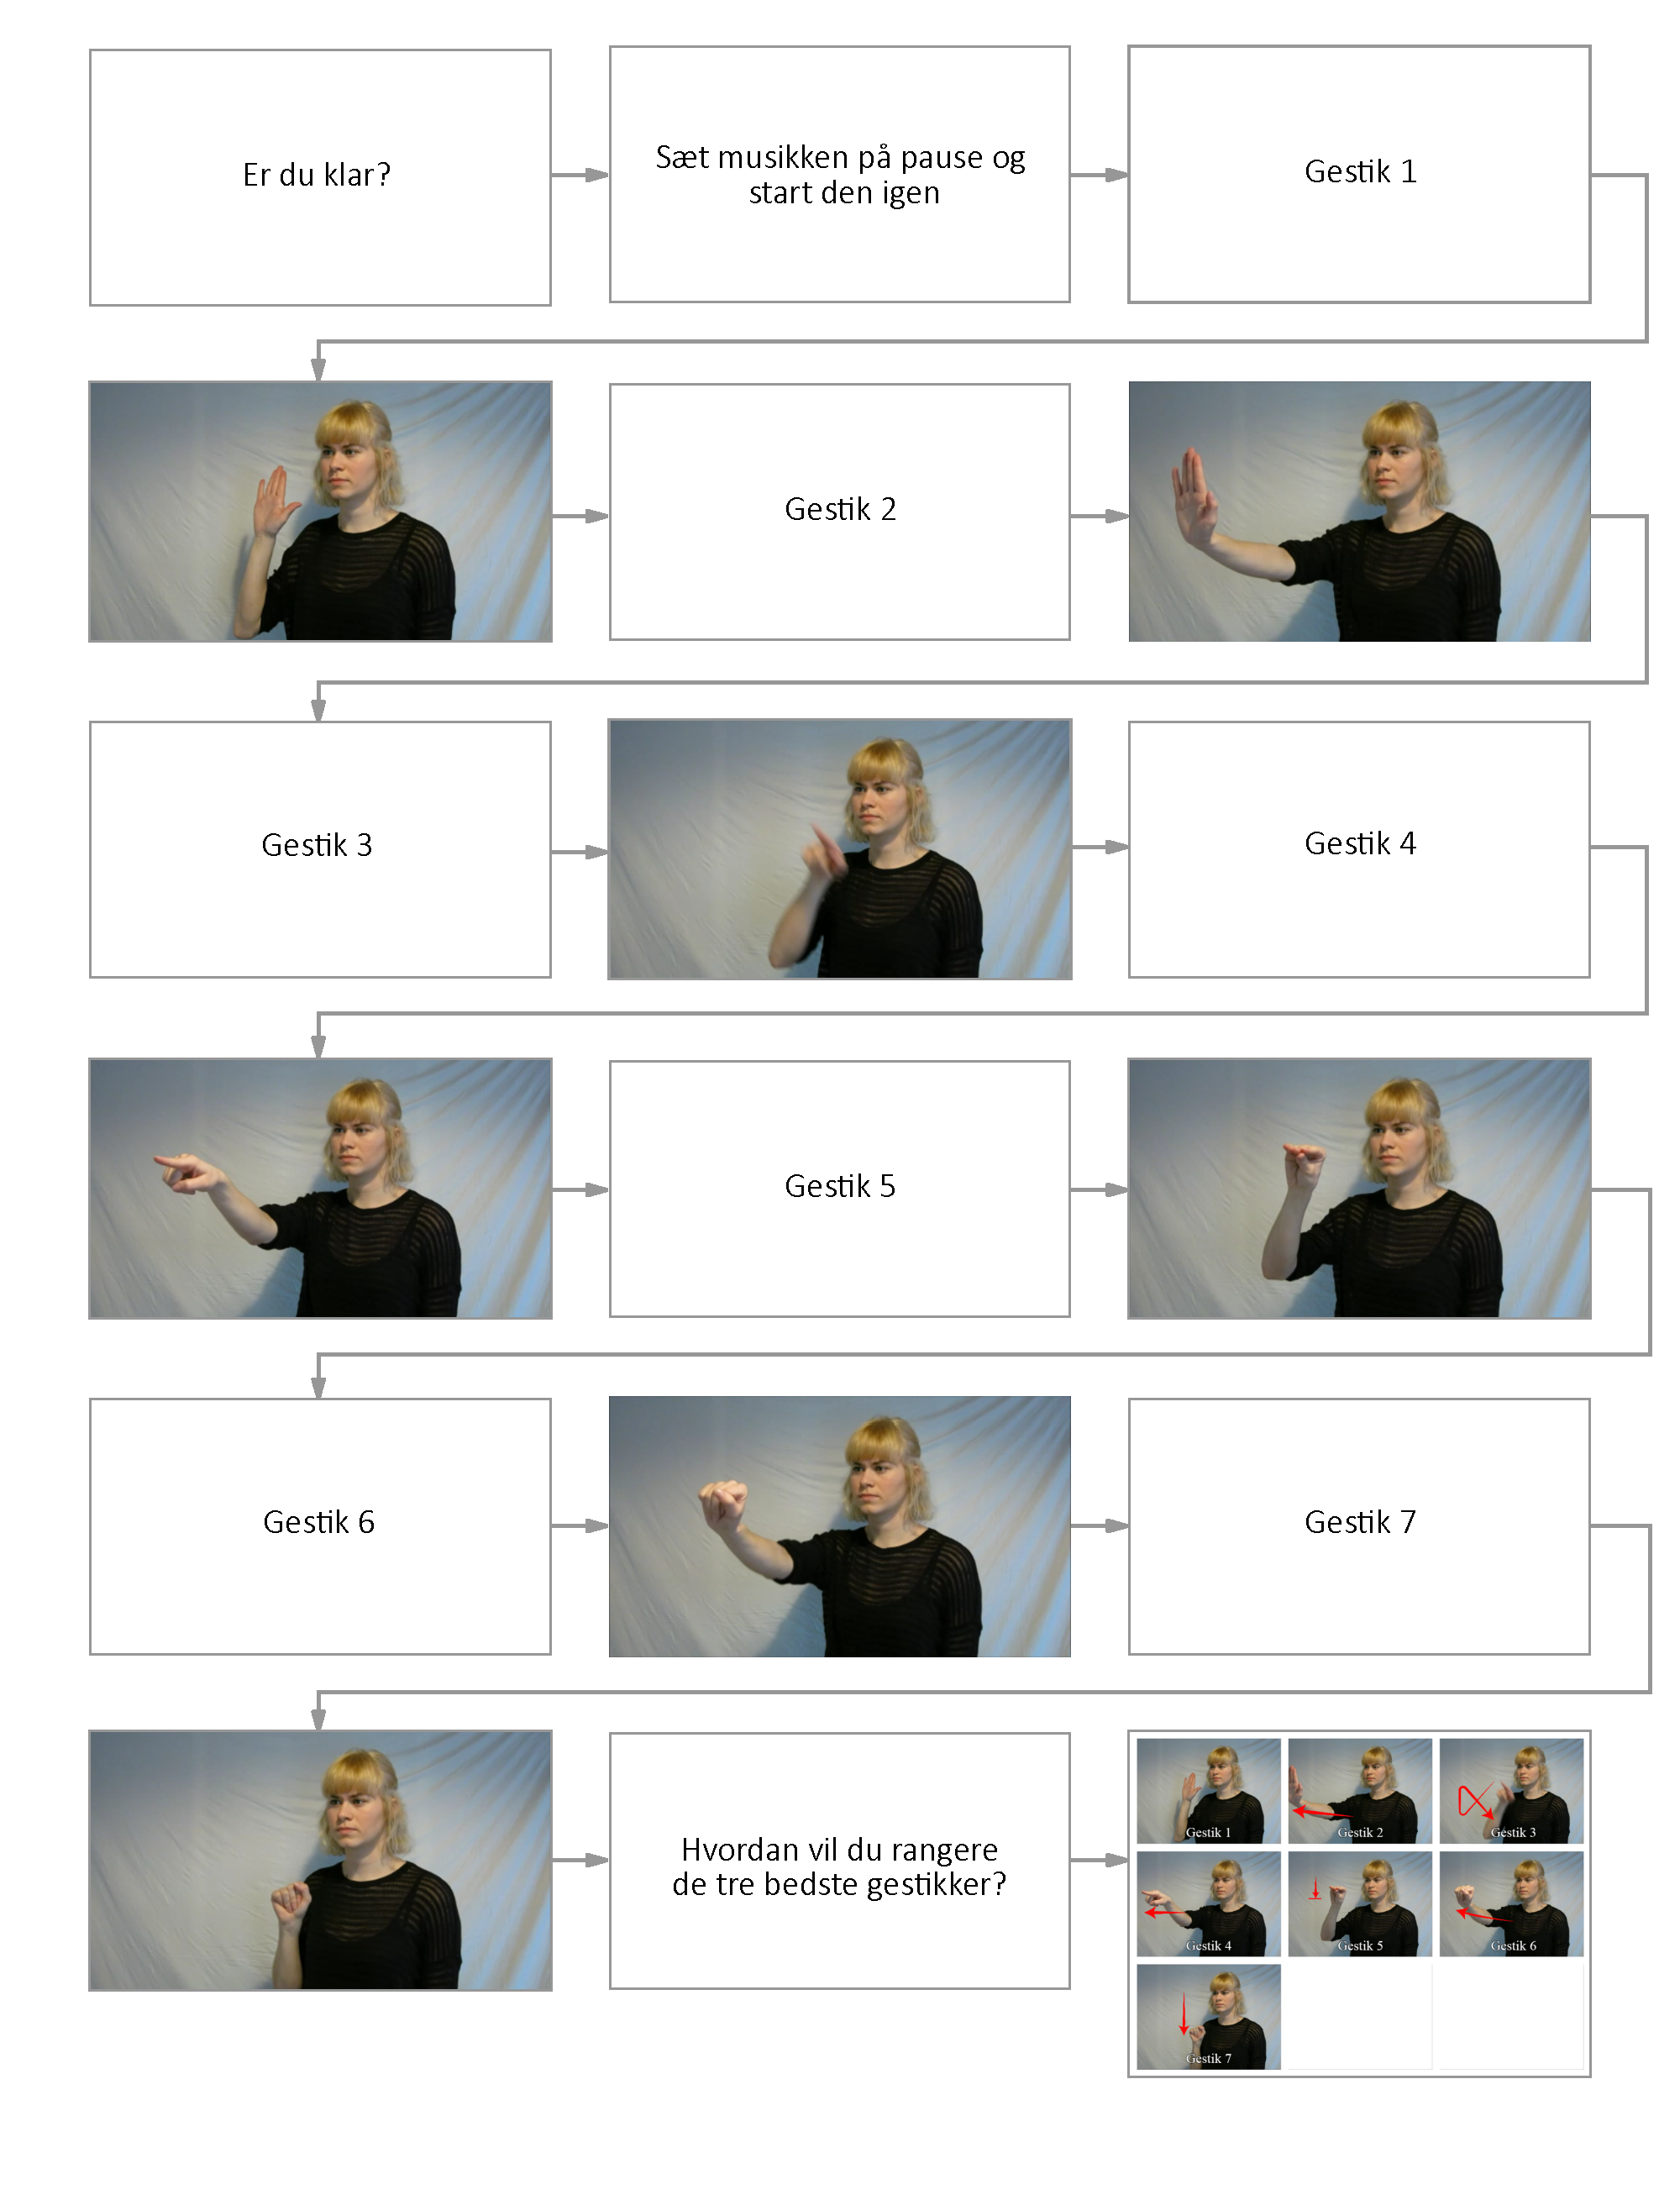
\includegraphics[resolution=300,width=\textwidth]{Flowdiagram/FlowdiagramPauseogStart}
	\caption{Ny.}
	\label{fig:FlowdiagramPause}
\end{figure}
\noindent
%

Her er de forskellige gestik-par blevet adskilt, hvorefter det er tydeliggjort hvornår hver ny gestik starter. Efter alle gestikker er demonstreret på videoen vises et oversigts-billede, hvor alle gestikkerne kan ses med nummerering og pile, der viser gestikkens retning. Disse tre oversigts-billeder er illustreret på \autoref{fig:OversigtPauseStart}, \autoref{fig:OversigtSkift} og \autoref{fig:OversigtVolumen}.
%
\begin{figure}[H]
	\centering
	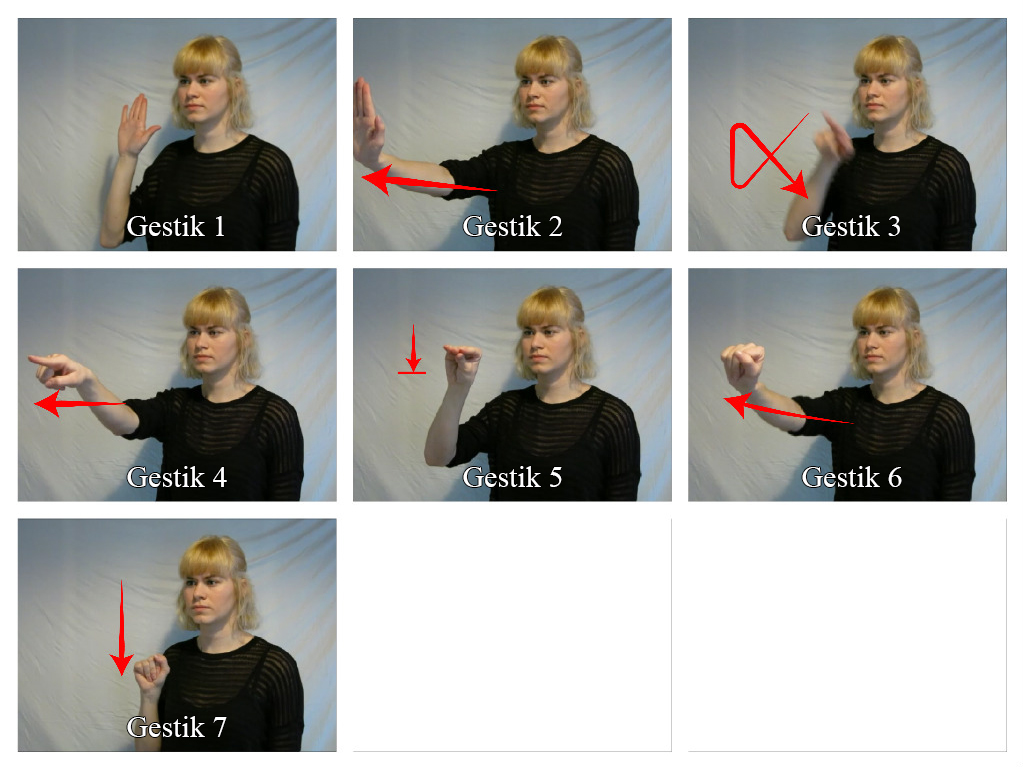
\includegraphics[resolution=300,width=\textwidth]{Test1/collage_start_pause_tekst}
	\caption{Opsummering af de syv semaforiske gestikker, der pauser og starter musikken, fra videoen, inklusiv nummerering og pile, som indikerer bevægelsesretning.}
	\label{fig:OversigtPauseStart}
\end{figure}
\noindent
%
%
\begin{figure}[H]
	\centering
	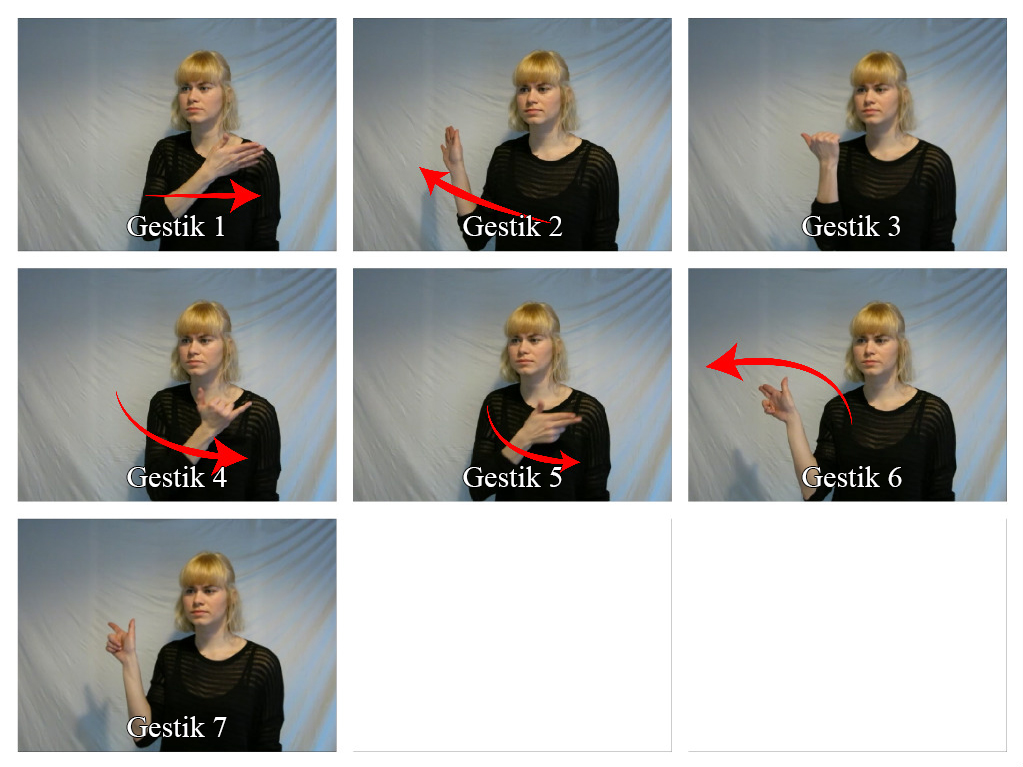
\includegraphics[resolution=300,width=\textwidth]{Test1/collage_Skiftsang_tekst}
	\caption{Opsummering af de syv semaforiske gestikker, der skifter musiknummer frem og tilbage, fra videoen, inklusiv nummerering og pile, som indikerer bevægelsesretning.}
	\label{fig:OversigtSkift}
\end{figure}
\noindent
%
%
\begin{figure}[H]
	\centering
	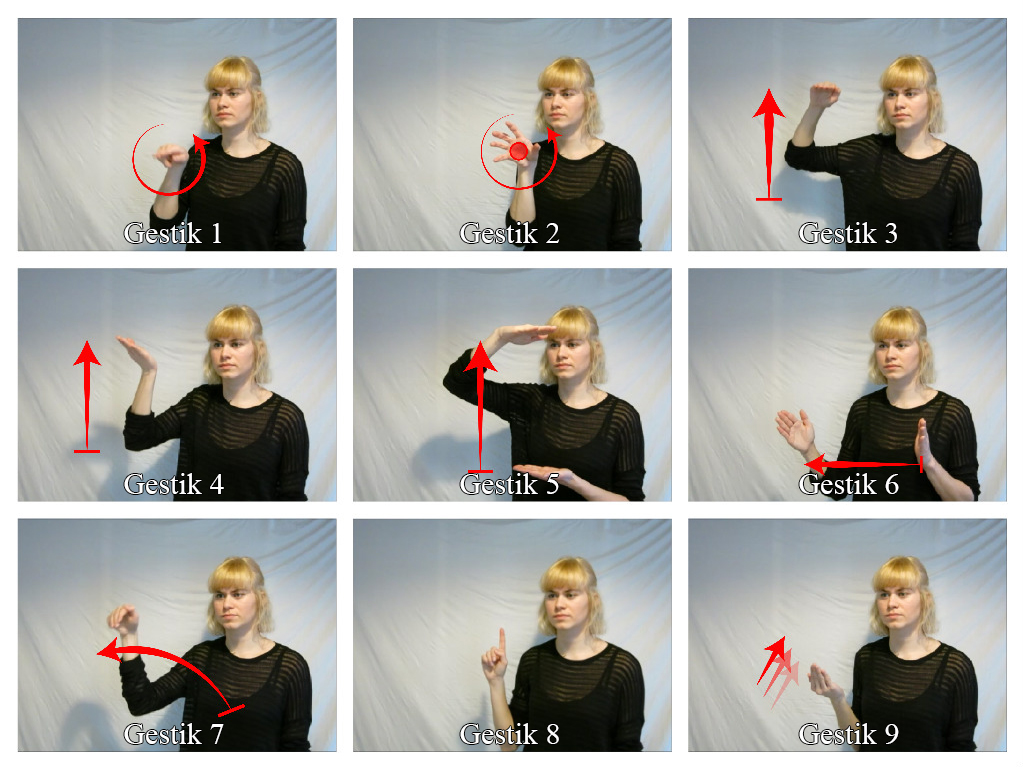
\includegraphics[resolution=300,width=\textwidth]{Test1/collage_volumen_tekst}
	\caption{Opsummering af de ni semaforiske gestikker til at skrue op og ned for musikken, fra videoen, inklusiv nummerering og pile, som indikerer bevægelsesretning.}
	\label{fig:OversigtVolumen}
\end{figure}
\noindent
%
